%!TEX program = xelatex
% Full chain: pdflatex -> bibtex -> pdflatex -> pdflatex
\documentclass[11pt,en,bibstyle=ieeetr]{elegantpaper}
\usepackage{algorithm}
\usepackage[noend]{algpseudocode}
\usepackage{listings}
\usepackage{color}

\definecolor{dkgreen}{rgb}{0,0.6,0}
\definecolor{gray}{rgb}{0.5,0.5,0.5}
\definecolor{mauve}{rgb}{0.58,0,0.82}

\lstset{frame=tb,
  language=Python,
  aboveskip=3mm,
  belowskip=3mm,
  showstringspaces=false,
  columns=flexible,
  basicstyle={\small\ttfamily},
  numbers=none,
  numberstyle=\tiny\color{gray},
  keywordstyle=\color{blue},
  commentstyle=\color{dkgreen},
  stringstyle=\color{mauve},
  breaklines=true,
  breakatwhitespace=true,
  tabsize=3
}


\title{OBProx-SG paper-recurrence-note}
\author{Zhenwei Lin}
% \institute{\href{https://github.com/ElegantLaTeX}{Elegant\LaTeX{} Program}}

% \version{0.08}
\date{\today}


\begin{document}

\maketitle

% \begin{abstract}
% This documentation illustrates the usage of the \href{https://github.com/ElegantLaTeX/ElegantPaper}{ElegantPaper} template. This template is based on the standard \LaTeX{} article class, which is designed for working paper writing. With this template, you can get rid of all the worries about the format and merely focus on writing. For any question, please leave a message on \href{https://github.com/ElegantLaTeX/ElegantPaper/issues}{Github::ElegantPaper/issues}. Want to know more about Elegant\LaTeX{} Templates? Please visit: \href{https://github.com/ElegantLaTeX}{https://github.com/ElegantLaTeX}.\par
% \keywords{Elegant\LaTeX{}, Working Paper, Template}
% \end{abstract}


\section{Model theories}

\subsection{MobileNetV1}
Many papers on small networks focus on only on size but do not consider speed.

A different approach for obtaining  small networks is shrinking, facotrizing or compressing pretained networks. Another method for training small networks is distillation which uses a larger net-work to teach a smaller network.

We then describe the MobileNet network structure and conclude with descriptions of the two model shrinking hyper-parameters width multiplier and resolution multiplier.
\subsubsection{MobileNet Architecture}

A standard convolution both filters and combines inputs into a new set of outputs in one step.

The depthwise separable convolution splits this into two layers, a separate layer for filtering and a separate layer for combining.\textbf{This factorization has the effect of drastically reducting computation and model size}

Now we analysis the different computational cost between the two convolution methods.

Input dimension is $ D_F \times D_F \times M $,where $ D_F $ is spatial width and height of a square input feature map, M is the number of input channels

A standard convolutional layer is parameterized by convolution kernel K of size $ D_K \times D_K \times M \times N $ where $ D_k $ is the spatial dimension of the kernel assumed to be square and M is number of input channels and N is the number of output channels as defined previously.

The output feature map for standard convolution assuming stride 1 and padding is computed as :

$$ 
G_{k,l,n} = \sum_{i,j,m}^{} K_{i,j,m,n}\cdot F_{k+i-1,l+j-1,m}
$$
so standard convolutions have the computational cost of :
$$ 
D_K \cdot D_K \cdot M \cdot N \cdot D_F \cdot D_F
$$

Now consider the second method is to use depthwise convolutions adn pointwise convolutions.

\textbf{Step1:} Depthwise convolution with one filter per input channel can be written as:
$$ 
\hat{G}_{k,l,m} = \sum_{i,j}^{} \hat{K}_{i,j,m}\cdot F_{k+i-1,l+j-1,m}
$$
where $ \hat{K} $ is the depthwise convolutional kernel of size $ D_K\times D_K\times M $,so the depthwise convolution has a computational cost of 
$$ 
D_K\cdot D_K\cdot M \cdot D_F \cdot D_F
$$

Depthwise convolution is extremely efficient relative to standard convolution.\textbf{However it only filters input channels, it does not combine them to create new features.}

\textbf{Step2}: Depthwise separable convolution. Using N $ 1\times 1 $ convolution kernels. And the cost is 
$$ 
M\cdot N \cdot D_F \cdot D_F
$$

By expressing convolution as two step process of filtering and combining we get a reduction in computation of :
$$ 
\frac{D_k\cdot D_k\cdot M\cdot D_F \cdot + M\cdot N\cdot D_F \cdot D_F}{D_K \cdot D_K\cdot M \cdot N \cdot D_F \cdot D_F   } = \frac{1}{N}+\frac{1}{{D_K}^2}
$$


\subsubsection{Network Structure and Training}

The MobileNet structure is built on depthwise separable convolutions as metioned in the previous section except for \textbf{first layer which is a full convolution.}

The MobileNet architecture is defined in Table \ref{table1}.
\begin{figure}[h]
\caption{MobileNet Body Architecture}
\begin{center}
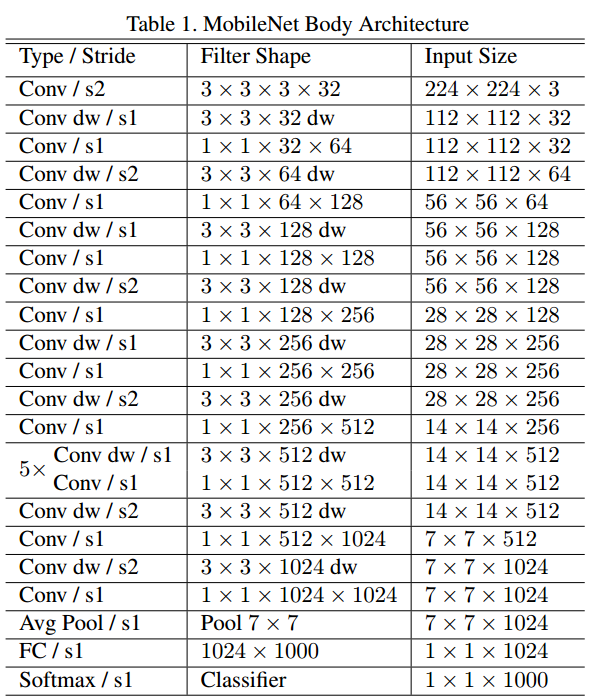
\includegraphics{table1.png}\label{table1}
\end{center}

\end{figure}

All layers are followed by a batchnorm and ReLU nonlineraity with the exception of the final fully connected layer which has no nonlinearity and feeds into a softmax layer for classification.

Figure \ref{comparison}contrasts a layer with regular convolutions, batchnorm and ReLU nonlinearity to the factorized layer with depthwise convolution, $ 1\times 1 $ pointwise convolution as well as batchnorm and ReLU after each convolutional layer.

\begin{figure}
	\centering
	\caption{comparison of A and B}
	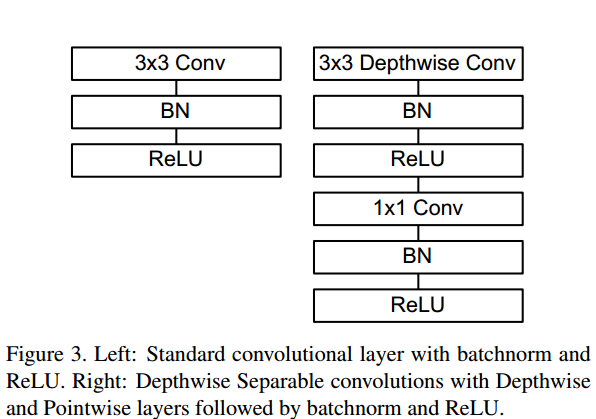
\includegraphics{fig/contrast.png}
\label{comparison}
\end{figure}

\textbf{Batchnorm:} is a method used to make artificial neural networks faster and more 
stable through normalization of the input layer by recentering and re-scaling. It was believed
that it can mitigate the problem of internal covariate shift, where parameter initialization and changes in the distribution of the inputs of each layer affect the learning rate of the  network.


\textbf{Motivation of Batchnorm: the phenomenon of internal covariate shift}

Each layer of a neural network has inputs with a corresponding distribution, which is 
affected during the training process by the randomness in the parameter initialization and the ranodmness in the input data.
The effect of these sources of randomness on the distribution of the inputs to interval layers during training is described as internal covariate shift.

(An important hypothesis in Machine learning: training data has the same distribution with test data; Then, refine to each layer of the neural network, the distribution is inconsistent in each round of training. Then the relative training effect cannot be guaranteed, so it is called covariate shift between layers. )


\textbf{Batch Normalizing Transform:}

Use B to denote a mini-batch of size m o fthe entire training set. The empirical mean and variance of B could thus be denoted as 
$$ 
\mu _B = \frac{1}{m}\sum_{i=1}^{m}x_i \quad \text{and}\quad \sigma ^2_B = \frac{1}{m}\sum_{i=1}^{m}(x_i-\mu _B)^2
$$

For a layer of the network with d-dimension input, $ x = (x^{(1)},\ldots, x^{(d)}) $,each dimension of its input is then normalized
$$ 
\hat{x}_i^{(k)} = \frac{x_i^{(k)}-\mu _{B}^{(k)}}{\sqrt{\sigma _{B}^{(k)^2}+\epsilon }}
$$
where $ k \in [1,d] $ and $ i \in [1,m] $, $ \epsilon  $ is added in the denominator for numerical stability and is and arbitrarily small constant.
The resulting normalized activation $ \hat{x}^{(k)} $ have zero mean and unit variance, if $ \epsilon $ is not taken into account.

\textbf{To restore the representation power of the network, a transformation step then follows as:}
$$ 
y_i^{(k)} = \gamma ^{(k)} \hat{x}_i^{(k)} + \beta^{(k)}
$$
where the parameter $ \gamma ^{(k)} $ and $ \beta ^{(k)} $ are subsequently learned in the optimization process.

Formally, the operation that implements batch normalization is a transform $ BN_{\gamma ^{(k)},\beta ^{(k)}}(x^{(k)}):x_{1\ldots m}^{(k)} \rightarrow y_{1 \ldots m}^{(k)} $ called batchnormalizing transform.

The reason of restoring the representation power of the network is a normalization make most of the activated values fall into the linear region of the nonlinear funciton. 
However, this method equals to replace nonlinear function with linear function, so the representation power of network is decreased.

Down sampling is handled with strided convolution in the depthwise convolutions as well as in the  first layer. A final average pooling reduces the spatial resolution to 1 before the fully connected layer.

Our model structure puts nearly all of the computation into dense $ 1\times 1 $ convolutions. This can be implemented with highly optimized general matrix multiply(GEMM) functions.

\subsubsection{Width Multiplier: Thinner Models}

Although the base MobileNet architecture is already small and low latency, many times a specific use case
or application may require the model to be smaller and faster.

\textbf{Width multiplier $ \alpha$} the role of the width multiplier $ \alpha$ is to thin a network \textbf{uniformly} at each layer.
For a given layer and width multiplier $ \alpha $ the number of input channels M becomes $ \alpha M$ and the output channels N becomes $ \alpha N $

The computational cost of a depthwise separable convolution with width multiplier $ \alpha$ is:
$$ 
D_K \cdot D_K \cdot \alpha M \cdot D_F \cdot D_F + \alpha M \cdot \alpha N \cdot D_F \cdot D_F
$$



\subsection{ResNet18}

\subsubsection{Introduction}
Driven by the significace of depth, a questiion arises: Is learning better networks as easy as stacking more layers?

An obstacle to answering this question was the notorious problem of vanishing/exploding gradients, which hamper convergence from the beginning. This problem, however, has been 
largely addressed by normalized initialization and itermediate normalizationlayers, which enable networks with tens of layers to start converging for 
stochastic gradient descent with back propagation.

When deeper networks are able to start converging, a degradation problem has been exposed: with the network
depth increasing, accuracy gets saturated (which might be unsurprising) and then degrades rapidly.
Unexpectedly, such degradation is not caused by  overfitting, and adding more layers to a suitably deep model leads to higher training error.

Let us consider a shallower architecture and its deeper counterpart that adds more layers onto it.
There existence of this constructed solution indicates that a deeper model should produce no higher training error
than its shallower counterpart.\textbf{But experiments show that our current solvers on hand are unable to find solutions that are comparably good or better than the constructed solution, or unable to do so in feasible time.}

In this paper, we address the degradation problem by introducing a deep residual learning framwork.
Instead of hoping each few stacked layers directly \textbf{fit a desired underlying mapping}, we explicitly let these layers fit a residual mapping.

Formally, denoting the desired underlying mapping as $ \mathcal{H}(x) $
we let the stacked nonlinear layers fit another mapping of 
$$ 
\mathcal{F}(x):=\mathcal{H}(x)-x
$$

To the extreme, if an identity mapping were optimal, it would be easier to \textbf{push the residual
to zero} than to fit an identity mapping by a stack of nonlinear layers. 

The formulation of $ \mathcal{F}(x)+x $ can be realized by feedforward neural network with "shortcut connections"(as being shown in figure \ref{res})
\begin{figure}
	\centering
	\caption{Residual learning: a building block}
	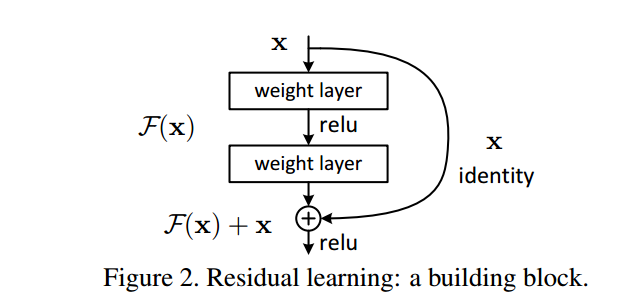
\includegraphics{fig/res.png}
	\label{res}
\end{figure} 

\subsubsection{Deep Residual Learning}
If the added layers can be constructed as identity mappings, a deeper model should have training
error no greater than its shallower counter-part. The degradation problem suggests that the solvers might have difficulties in approximating identity mappings by multiple nonlinear layers.

With the residual learning reformulation, if identity mappings are optimal, the solvers may 
simply drive the weights of the multiple nonlinear layers toward zero to approach identity mappings.

In real cases, it is unlikely that identity mapping are optimal, but our reformulation may help 
to precondition the problem.
The experiments show that the learned residual functions in general have small responses, suggesting that identity mappings provide reasonable preconditioning.

\textbf{Identity Mapping by shortcuts:}

We consider a building block defined as: 
$$ 
y = \mathcal{F}(x,\left\{ W_i \right\} )+x
$$
where x and y are the input and output vectors of the layers considered.
The function $ \mathcal{F}(x,\left\{ W_i \right\} ) $ represents the residual mapping to be learned.
The operation $ \mathcal{F}+x$ is performed by a shortcut connection and element-wise addition.
The shortcut connections introduce neither extra parameter nor computation complexity. This is not only
attractive in practice but also important in our comparisons between plain and residual networks.
that simultaneously have the same number of parameters, depth, and computational cost.

The dimension of x and $ mathcal{F} $ must be equal, in this is not the case(e.g., when changing the input/output channels),
we can perform a \textbf{linear projection $ W_s $ }by the shortcut connections to match the dimensions:
$$ 
y = \mathcal{F}(x,\left\{ W_i \right\} )+W_s x
$$
We can also use a  square matrix $ W_s $, but we will show by experiments that the identity mapping
is sufficient for addressing the degradation problem and is economical and \textbf{thus $ W_s $ is only used when matching dimensions.}
The function $ \mathcal{F}(x,\left\{ W_i \right\} ) $ can represent multiple convolutional layers. The element-wise addition is performed
on two feature maps, channel by channel.

\subsubsection{Network Architectures}
We have tested various plain/residual nets, and have observed consistent phenomena.

\textbf{Plain Network:} inspired by the philosophy of VGG net. The convolutional layers mostly have $ 3\times 3 $filter and follow two simple 
design rules:
\begin{enumerate}
		\item for the same output feature map size, the layers have the same number of filters;
		\item if the feature map size is halved, the number of filters is doubled so as to preserve the time complexity per layer. We perform downsampling directly convolutional layers that have a stride of 2.
\end{enumerate}

\textbf{Residual Network:}Based on above plain network, we insert shortcut connections as shown in Figure~\ref{res_net_str} right which turn the network into its counterpart residual version.

The identity can be directly used when the input and output are of the same dimensions (solid line shortcuts in Figure~\ref{res_net_str})
When the dimension increase (dotted line shortcuts in Figure~\ref{res_net_str}),we consider two options(This is very important and the second option was used in Orthant based's code)
\begin{enumerate}
	\item The shortcut still performs identity mapping, with extra zero entries padded for increasing dimensions. This option introduces no extra parameter.
	\item The projection shortcut in is used to match dimensions (done by $ 1\times 1$ convolutions)
\end{enumerate}
For both options, when the shortcuts go across feature maps of two sizes, they are performed with a stride of 2.

\begin{figure}
	\centering
	\caption{example network architectures for ImageNet}
	\label{res_net_str}
	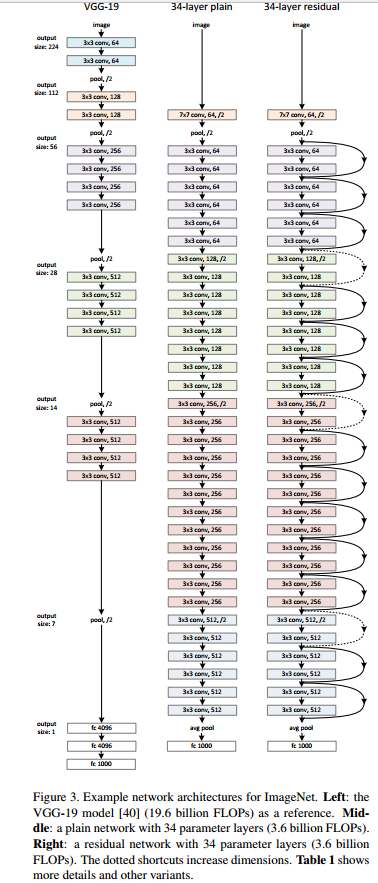
\includegraphics{fig/res_net_structure.png}
\end{figure}

\textbf{ImageNet Classification}

\textbf{Plain Network:}We first evaluate 18-layer and 34-layer plain nets . The 34-layer plain net is in Figure~\ref{res_net_str}
See Figure~\ref{detailed_archi} for detailed architectures.

\begin{figure}
	\centering
	\caption{plain network detailed architectures}
	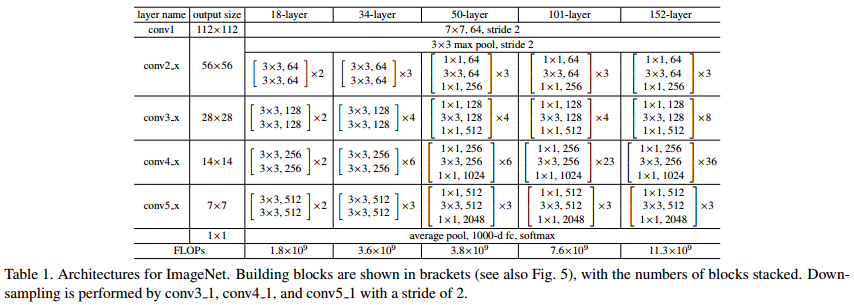
\includegraphics[width = 19cm]{fig/architectures.png}
\label{detailed_archi}
\end{figure}

\textbf{Residual Networks:} Next we evaluate 18-layer and 34-layer residual nets(ResNets).
The baseline architectures are the same as the above plain nets, expect that a shortcut connection is added to each pair of $ 3\times 3$ filters as in Figure~\ref{res_net_str}.
We use identity mapping 

\textbf{CIFAR-10 and Analysis}

The plain/residual hitectures follow the form in Figure~\ref{res_net_str} (middle/right). The network inputs are $ 32\times 32 $ images, with the per-pixel mean subtracted.






\section{DC approximation approaches: consistency results}

We focus on the sparse optimization problem with $l_0-$norm in the objective function,
called the $l_0-$problem, that takes the form
\begin{equation}
min \left\{ F(x,y) = f(x,y)+ \lambda \left\| x \right\| _0:(x,y) \in K\right\}
\label{primal_problem}
\end{equation}

where $\lambda $ is a positive parameter.K is a convex set in $\mathbb{R}^{n}\times \mathbb{R}^m$ and $f$  is a finite DC function on  $\mathbb{R}^n \times \mathbb{R}^m$. Suppose that $f$ has a DC decomposition 
$$ f(x,y) = g(x,y) - h(x,y)\quad \forall (x,y) \in \mathbb{R}^n\times \mathbb{R}^m$$    

where $g,h$ are finite convex funtion on $ \mathbb{R}^n \times \mathbb{R}^m$.

Define the step functions: $\mathbb{R} \rightarrow \mathbb{R}$ by $s(t) = 1$ for $t \neq 0$  and $s(t)= 0$ 

\begin{equation*}
s(t) = \left\{
	\begin{array}{l}
		1\quad t \neq 0\\
		0\quad otherwise
	\end{array}\right.
\end{equation*}

Then $\left\| x \right\| _0 = \sum_{i=1}^{n}s(x_i)$, the idea is to replace the discontinuous step function by a continuous approximation $r_\theta$, where $\theta>0$ is a parameter controling the tightness of approximation.

Assumption:$\left\{ r_\theta \right\}_{\theta >0} $ is a family of funciton $\mathbb{R} \rightarrow \mathbb{R}$ satifying the folling properities: 

\begin{enumerate}
	\item $\lim_{\theta \to +\infty}r_\theta(t) = s(t),\forall t \in \mathbb{R}$  
	\item $\forall \theta>0$,$r_\theta$ is even, i.e.$r_\theta (\left| t \right| ) = r_\theta(t)(\forall t \in \mathbb{R})$ and $r_\theta$ is a increasing on $[0,+\infty)$    
	\item $ \forall \theta >0 $, $ r_\theta $ is a DC function which can be represented as $ r_\theta (t) = \varphi_\theta(t)-\psi_\theta(t), t \in \mathbb{R}$,where $ \varphi_\theta,\psi_\theta $ are finite convex functions on $ \mathbb{R} $
	\item $ t\mu \geq 0, \forall t \in \mathbb{R} , \mu \in \partial r_\theta(t)$, where $ \partial r_\theta(t) = \left\{ u-v:u \in \partial r_\theta(t) ,v \in \partial\psi_\theta(t)\right\} $  
	\item $ \forall a \leq b $ and $ 0 \not\in [a,b] $,then $ \lim_{\theta \to \infty }sup \left\{ \left| z \right| :z \in \partial r_\theta(t),t \in [a,b] \right\} = 0 $
\end{enumerate}

First of all, we observe that by assumption 2 above, we get another equivalent form of 
\begin{equation}
	\min_{(x,y,z) \in \Omega_1} \bar{F}_{r_\theta}(x,y,z) :=f(x,y)+\lambda \sum_{i=1}^{n}r_{\theta }(z_i)
\label{approximate_problem}
\end{equation}

where $ \Omega_1 = \left\{ (x,y,z):(x,y) \in K, \left| x_i \right| \leq z_i,\forall i=1,...,n\right\}  $

Indeed,\ref{primal_problem} and \ref{approximate_problem} are equivalent in the following sense.

\begin{proposition}



	A point $ (x^*,y^*) \in K $ is a global(resp.local) solution of the problem \ref{primal_problem} if and only if $ (x^*,y^*,\left| x^* \right| ) $ is a global (resp.local) solution
	of the problem \ref{approximate_problem}. Moreover , if $ (x^*,y^*,z^*) $ is a global solution of \ref{approximate_problem},then ($ x^*,y^* $) is a global solution of \ref{primal_problem}
\end{proposition}
\begin{proof}
	There are many problem in the proof process. 
	Since $ r_\theta $ is an increasing function on $[0,+\infty)$, we have $$ \bar{F}_{r_\theta}(x,y,z) \geq \bar{F}_{r_\theta}(x,y,\left| x \right| ) = F_{r_\theta}(x,y) $$
the inequality by $ \Omega_1 = \left\{ (x,y,z):(x,y) \in K, \left| x_i \right| \leq z_i \right\}  $
\end{proof}


Now we show the link between the original problem and the approximate problem. This result gives a mathmatical foundation of approximation methods.

\begin{theorem}
	Let $ \mathcal{P},\mathcal{P}_\theta $ be the solution sets of the problem \ref{primal_problem} and \ref{approximate_problem} respectively.
	\begin{enumerate}
		\item Let $ \left\{ \theta_k \right\}$ be a sequence of nonnegative numbers such that $ \theta_k \to + \infty $ and
			$ \left\{ (x^k,y^k) \right\}  $ be a sequence such that $ (x^k,y^k) \in \mathcal{P}_{{\theta}_k} \forall k$. If 
			$ (x^k,y^k) \to (x^*,y^*) $,then $ (x^*,y^*) \in \mathcal{P}$
		\item If $ K $ is compact, then $ \forall \epsilon >0 $, there is $ \theta(\epsilon)>0 $,such that  $ \mathcal{P}_{\theta} \subset \mathcal{P}+B(0,\epsilon) ,\forall \theta \geq \theta(\epsilon )$
		\item If there is a finite set S such that $  \mathcal{P}_{\theta} \bigcap S \neq 0 \forall \theta >0 $, then there exits $ \theta_0 \geq 0 $ such that $$ \mathcal{P}_{\theta} \bigcap S \subset \mathcal{P} \quad \forall \theta \geq \theta_0$$
	\end{enumerate}
\end{theorem}

\begin{proof}
	Let (x,y) be arbitrary in K. For any k, since $ (x^k,y^k) \in \mathcal{P}_{\theta_k} $,
	we have 
	$$
	f(x,y) + \lambda \sum_{i=1}^{n}r_{\theta_k}(x_i) \geq f(x^k,y^k)+\lambda \sum_{i=1}^{n}r_{\theta_k}(x_i^k) 
	$$v
because $ \mathcal{P}_{{\theta}_k} $ is the solution sets of problem \ref{approximate_problem}

By assumption 2:
 $\forall \theta>0$,$r_\theta$ is even, i.e.$r_\theta (\left| t \right| ) = r_\theta(t)(\forall t \in \mathbb{R})$ and $r_\theta$ is a increasing on $[0,+\infty)$
 
 If $ x_i^* = 0$, we have $ \liminf\limits _{k \to + \infty} r_{\theta_k}(x_i^k) \geq \liminf\limits_{k\to +\infty}{r_{\theta_k}}(0) = 0$. (so the limit point $ (x^*,y^*) $ is minimum)
 
 If $ x_i^* \neq 0 $, there exists $ a_i \leq b_i $ and $ k_i \in \mathbb{N} $ such that $ 0 \notin [a_i,b_i] $ and $ x_i^k \in [a_i,b_i] $ for all $ k \geq k_i $. 
 Then we have 
$$ 
\left| r_{\theta_k}(x_i^k) - s(x_i^*) \right| \leq max \left\{\left| r_{\theta_k}(a_i)-s(a_i) \right|,\left| r_{\theta_k}(b_i)-s(b_i) \right|    \right\}  \forall k \geq k_i
$$
(concave funciton substract 1, and get its absolute value, so need to get maximum)

Since $ \lim_{k \to \infty} r_{\theta_k}(a_i) = s(a_i)$ and $ \lim_{k \to \infty} r_{\theta_k}(b_i) = s(b_i)  $,we have $ \lim_{k \to \infty}r_{\theta_k}(x_i^k)  = s(x_i^*) $

Note that $ f $ is continuous, takeing liminf of both side of $f(x,y) + \lambda \sum_{i=1}^{n}r_{\theta_k}(x_i) \geq f(x^k,y^k)+\lambda \sum_{i=1}^{n}r_{\theta_k}(x_i^k) 
 $ 
we have 
$$ 
f(x,y)+\lambda \sum_{i=1}^{n}s(x_i) \geq f(x^*,y^*) + \liminf\limits_{k \to \infty}r_{\theta_k}(x_i^k) = f(x^*,y^*) + \lambda \sum_{i=1}^{n}s(x_i^*)
$$
Thus, $ F(x,y) \geq F(x^*,y^*) \forall (x,y) \in K$ or $ (x^*,y^*) \in \mathcal{P} $
\end{proof}

\begin{proof}
	Consider its contradiction is $ \exists \epsilon >0, \forall \theta(\epsilon)>0, \exists \theta > \theta(\epsilon)$ such that $\mathcal{P}_\theta \nsubseteq \mathcal{P}+B(0,\epsilon ) $	

	so there $ \exists \epsilon$  without loss of generality,$ \forall \theta_1(\epsilon )>0$
$ \exists \theta _2(\epsilon) > \theta_1(\epsilon) $ such that $ P_{\theta_2} \nsubseteq P+B(0,\epsilon) $
.let $ \theta_2 $ replace $ \theta_1 $, then we can get $ \theta_3 $ meet the above conditions. So we can get a subsequence converge in out of $ P+B(0,\epsilon) $,
but this is an infinity sequence, so its limit point is should converges to compact set K($ P_{\theta_k} $) which is a contradiction.
\end{proof}

\begin{proof}
	Consider its contradiction is $ \forall \theta_0 $, there $ \exists \theta > \theta_0 $ such that $ P_\theta \bigcap S \nsubset P$.
	
	Next let $ \theta_1 $ replace $ \theta$, so it can generate a infinity sequence by this method, so there exists $ (x_i,y_i) \in P_{\theta_i} \bigcap S $ and $ \not\in P $ but $ \left\{ (x_i,y_i)_{i=1,2,3,...} \right\} \subseteq S $, 
	
	because $ \left\{ (x_i,y_i) \right\}  $ is a infinity sequence and S is a finite set, so the sequence would converge to a point $ (\bar{x},\bar{y}) $, by 1 ,this point should $ \not\in P $ which contradict to the $ (x^*,y^*) \in P $. 
\end{proof}








\section{Programming Syntax}

Now we introduce the Syntax by Adam algorithm 
 \begin{algorithm}[H]
        \caption{Outline of Adam}\label{alg1}
        \begin{algorithmic}[1]
            \Procedure{Adam}{$\alpha,\beta_1,\beta_2$}\newline
			\textbf{Input:} $ \alpha = 0.001,\beta_1 = 0.9,\beta_2 = 0.999$ and $ \epsilon = 10^{-8} $ where $ \beta_1,\beta_2 $ are exponential decay rates for the moment estimates
			\State{\textbf{Initialize:}  $ \theta_0,m_0,v_0,t$}\newline
			where $\theta_0 $ is parameter vector; $ m_0$  1-st moment vector; $ v_0 $ 2-nd moment vector; t is timestep.
			\While{$ \theta_t $ not converged }
			\State{$ t \leftarrow t+1 $}
			\State{$ g_t \leftarrow \nabla_{\theta}{f_t(\theta_{t-1})} $}
			\State{$ m_t \leftarrow \beta_1 m_{t-1}+(1-\beta_1)g_t $}
			\State{$ v_t \leftarrow \beta_2 v_{t-1}+ (1-\beta_2)g_t\bigodot g_t $}
			\State{$ \hat{m}_t \leftarrow m_t/(1-\beta _1^t)$(Compute bias-corrected first moment estimate, t power)}
			\State{$ \hat{v}_t \leftarrow v_t/(1-\beta _2^t) $(Compute bias-corrected second raw moment estimate, t power)}
			\State{$ \theta_t \leftarrow \theta_{t-1} - \alpha \cdot \hat{m}_t/(\sqrt{\hat{v}_t}+\epsilon) $(Update parameters)}
			\EndWhile
			\State{\textbf{return} $ \theta_t $(Resulting parameters)}
            \EndProcedure
        \end{algorithmic}
        \label{alg_1}
    \end{algorithm}



Some basic starters

The \textbf{params} are model's parameters, and the parameter \textbf{defaults} need to update in the algorithm.
\subsection{About initializing parameter}
\begin{lstlisting}
	def __init__(self,params,lr,betas = (0.9,0.99)):
		if not 0.0 <= lr:
			raise ValueError("Invalid learning")
		defaults = dict(lr = lr,betas = betas)
		super(algorithm_name,self).__init__(params,defaults)
\end{lstlisting}

Key is step function, and it need to be decorated by \textbf{torch.no\_grad()}
\begin{lstlisting}
	@torch.no_grad()
	def step(self, closure = None):
		'''
		closure(callable,optional): A closure that reevaluates the model and return the loss
		'''
		loss = None #first put loss to None, and it will recalculate.
		if closure is not None:
			with torch.enable_grad():
				loss = closure()

\end{lstlisting}
Some basic formulas.
Note that there is "is None"
\begin{lstlisting}
	@torch.no_grad()
	def step(self, closure = None):
		'''
		closure(callable,optional): A closure that reevaluates the model and return the loss
		'''
		loss = None #first put loss to None, and it will recalculate.
		if closure is not None:
			with torch.enable_grad():
				loss = closure()
		for group in self.param_groups:
			'''
			There are some hyperparameters you can get here which is from outside.
			'''
			lr = group['lr']
			beta1,beta2 = group['betas']
			for p in group['params']:
				'''Next is about how to change p which is model's parameter'''
				if p.grad is None:
					continue
\end{lstlisting}

And we will find the iteration will using the information from the last iteration.
So you need to use container to hold it, like \textbf{state}

\begin{lstlisting}
state = self.state[p]

#State initialization
if len(state) == 0:
	state['step'] = 0
	#Exponential moving average of gradient values,which is $m_t$ in the formula 
	state['exp_avg'] = torch.zeros_like(p,memory_format = torch.preserve_format)
	#Exponential moving average of squared gradient values, which is $v_t$ in the formula
	state['exp_avg_sq'] = torch.zeros_like(p,memory_format = torch.preserve_format)

\end{lstlisting}

\begin{lstlisting}
import math
import torch
from .optimizer import Optimizer
class adam(Optimizer):
    def __init__(self,params,lr = 1e-3, betas = (0.9,0.999),eps = 1e-8):
        if not 0.0 <= lr:
            raise ValueError('Invalid learning rate: {}'.format(lr))
        if not 0.0 <= eps:
            raise ValueError('Invalid epsilon value: {}'.format(eps))
        if not 0.0 <= betas[0]<1.0:
            raise ValueError('Invalid beta parameter at index 0: {}'.format(betas[0]))
        if not 0.0 <= betas[1]<1.0:
            raise ValueError('Invalid beta parameter at index 0: {}'.format(betas[1]))
        defaults = dict(lr = lr,betas = betas,eps = eps)
        super(adam,self).__init__(params, defaults)
        
    @torch.no_grad()
    def step(self,closure = None):
        loss = None
        if closure is not None:
            with torch.enable_grad():
                loss = closure()
        
        for group in self.param_groups:
            lr = group['lr']
            beta1,beta2 = group['betas']
            eps = group['eps']
            for p in group['params']:
                if p.grad is None:
                    continue
                grad = p.grad

                state = self.state[p]
                if len(state) == 0:
                    state['step'] = 0
                    state['m'] = torch.zeros_like(p,memory_format=torch.preserve_format)
                    state['v'] = torch.zeros_like(p.memory_format=torch.preserve_format)
                
                m = state['m']
                v = state['v']
                # t+1
                state['step'] += 1
                m.mul_(beta1).add_(grad,alpha = 1-beta1)
                # addcmul performs the element-wise multiplication of tensor1 by tensor2, multiply the result by the scalar value and add it to input.
                # out_i = input_i + value*tensor1_i*tensor2_i
                v.mul_(beta2).addcmul_(grad,grad,value = 1-beta2)

                bias_correction1 = 1- beta1**state['step']
                bias_correction2 = 1- beta2**state['step']

                hat_m = torch.div(m,bias_correction1)
                hat_v = torch.div(v,bias_correction2)

                denom = hat_v.sqrt().add_(eps)
                p.addcdiv(hat_m,denom,value = -lr)
        return loss
\end{lstlisting}

And you will find the code is different from official code, maybe official code is optimized in memory resource \textbf{which is needed to confirmed with the teacher.}


Next I consider a algorithm from the paper \href{https://arxiv.org/abs/1612.06265#:~:text=We%20consider%20a%20class%20of,and%20a%20continuous%20concave%20function.}{A proximal difference of convex algorithm with extrapolation} 
and the penalty function is $ r_{exp} = 1-\exp \left\{  -\theta \left| t \right|  \right\} $
and $ P_1 = \theta \left| t \right|  $, $ P_2 = \theta \left| t \right| + exp \left\{-\theta \left| t \right| \right\} -1 $


 \begin{algorithm}[H]
        \caption{Proximal difference of convex algorithm with extrapolation ($ pDCA_e $) for $ r_{exp} $}\label{alg2}
        \begin{algorithmic}[1]
            \Procedure{$ pDCA_e $}{L = lr}\newline
			\textbf{Input:}	$ \theta $(which is to the degree of controling approximation)\newline
				L(lr:learning rate),\newline
				$ x_0 \in dom P_1 $ \newline
				$\left\{ \beta_t \right\} \subset [0,1) $ with $ \sup_t \beta_t <1 $,\newline
				set $ x^{-1} = x^0 $
			\State{\textbf{Initialize:}$ k_{-1} = k_{0} = 1 $}
			\While{$ x_t $ is not convergence}
			\State{$ \xi ^t = sign(x^t) \theta(1-exp \left\{ -\theta \left| x^t \right|  \right\} ) $}
		
			\State{$ \beta _t = (k_{t-1}-1)/k_t$}
	\State{$ k_{t+1} = (1+\sqrt{1+4k_t^2})/2 $}
			\State{$ y_t = x_t + \beta _t(x_t-x_{t-1}) $}
			\State{
				\begin{equation*}
				x_{t+1} = \left\{
					\begin{array}{cl}
						-\frac{1}{L}(\nabla{f(y_t)} - \xi ^t+\theta)+y_t&,y_t>\frac{1}{L}(\nabla{f(y^t)}-\xi^t+\theta)\\
						0&,\text{otherwise}\\
						-\frac{1}{L}(\nabla{f(y_t)}-\xi ^t-\theta)+y_t&,y_t<\frac{1}{L}(\nabla{f(y_t)}-\xi^t-\theta)
					\end{array}\right.
				\end{equation*}}
				\State{$ t\leftarrow t+1 $}
			\EndWhile
            \EndProcedure
        \end{algorithmic}
        \label{alg_2}
    \end{algorithm}














% \textbf{Note:} ElegantPaper is available on  \href{https://www.overleaf.com/latex/templates/elegantpaper-template/yzghrqjhmmmr}{Overleaf} and \href{https://gitee.com/ElegantLaTeX/ElegantPaper}{gitee}.

% \subsection{Global Options}
% Language mode option \lstinline{lang} allows two alternative inputs, \lstinline{lang=en} (default)  for English or \lstinline{lang=cn} for Chinese. \lstinline{lang=cn} will make the caption of figure/table, abstract name, refname etc. Chinese. You can use this option as
% \begin{lstlisting}
% \documentclass[lang=cn]{elegantpaper} % or
% \documentclass{cn}{elegantpaper} 
% \end{lstlisting}
% \textbf{Note:} Under the English mode \lstinline{lang=en}, Chinese characters are not allowed. To type in Chinese, please load  \lstinline{ctex} or \lstinline{xeCJK} package at the preamble as:
% \begin{lstlisting}
% \usepackage[UTF8,scheme=plain]{ctex}
% \end{lstlisting}

% \subsection{Fonts}
% This template sets \lstinline{newtxtext} and \lstinline{newtxmath} for English and math fonts respectively.
% \begin{equation}
% (a+3b)^{n} = \sum_{k=0}^{n} C_{n}^{k} a^{n-k} (3b)^k\label{eq:binom}
% \end{equation}

% \subsection{Custom Commands}
% Default \LaTeX{} commands and environments are all the same in this template\footnote{To ensure the codes are replicatable. We recommend users pay more attention to the contents other than formats. This is the meaning of the existence of the template.}. We created four new commands:
% \begin{enumerate}
% 	\item \lstinline{\email}: create the hyperlink to email address.
% 	\item \lstinline{\figref}: same usage as \lstinline{\ref}, but start with label text <\textbf{Figure n}>.
% 	\item \lstinline{\tabref}: same usage as \lstinline{\ref}, but start with label text <\textbf{Table n}>.
% 	\item \lstinline{\keywords}: create the keywords in the abstract section.
% \end{enumerate}


% \subsection{Bibliography}
% This template used \hologo{BibTeX} to generate the bibliography, the default bibliography style is  \lstinline{aer} under the option \lstinline{lang=en}. Citation example: ~\citep{en1,en2,en3} used data from a major peer-to-peer lending marketplace in China to study whether female and male investors evaluate loan performance differently. 

% If you want to use \hologo{BibTeX}, you must create a file named \lstinline{wpref.bib}, and add bib items (from Google Scholar, Mendeley, EndNote, and etc.) to \lstinline{wpref.bib} file, and cite the bibkey in the \lstinline{tex} file. Note that \hologo{BibTeX} has to be added.

% Three options for the references, \lstinline{cite=numbers} (default), \lstinline{cite=super} and \lstinline{cite=authoryear}. Those who major in science and engineering use \lstinline{numbers} and \lstinline{super} more often, while those who major in arts use \lstinline{authoryear} more frequently. To switch different options, use
% \begin{lstlisting}
% \documentclass[cite=super]{elegantpaper} % super style ref style
% \documentclass[super]{elegantpaper}

% \documentclass[cite=authoryear]{elegantpaper} % author-year ref style
% \documentclass[authoryear]{elegantpaper}
% \end{lstlisting}

% \section{Recruit Support Members}

% Recruit support members for Elegant\LaTeX{} to translate template official guide, maintain wiki entries(Markdown), update Wechat articles. No deadline for this recruitment.

% So far, Elegant\LaTeX{} has four support members:
% \begin{itemize}
% 	\item OG Translator: \href{https://github.com/peggy2006xzyz}{YPY};
% 	\item Wiki Maintainer: \href{https://github.com/izinngo}{Ingo Zinngo}, \href{https://github.com/xiaohao890809}{Xiaohao890809};
% 	\item QQ Group Manager: \href{https://github.com/sikouhjw}{Sikouhjw}.
% \end{itemize}

% Thank them all!!!

% \section{Acknowledgement}
% The number of stars on Github for ElegantPaper reached 164 on Oct 17, 2019 at the release of ElegantPaper v0.08.
% Thank China\TeX{} and \href{http://www.latexstudio.net/}{\LaTeX{} studio} for their promotion. 

% If you like our templates, star on Github.
% \begin{figure}[!ht]
% 	\centering
% 	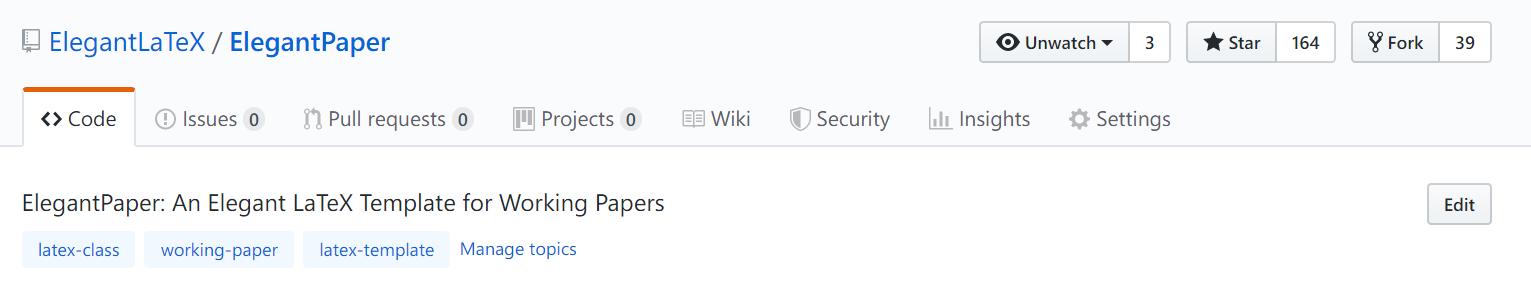
\includegraphics[width=\textwidth]{star.png}
% 	\caption{Twinkle, Twinkle, Little Star}
% \end{figure}

% \section{Donation}
% To express your love for our templates and/or our developers, please do not hesitate to tip us.
% \begin{figure}[!htbp]
% 	\centering
% 	
\includegraphics[width=0.4\textwidth]{donate.jpg}
% \end{figure}

% \textbf{The explanation right of the tip usage belongs to Elegant\LaTeX{} with no supervision. Feel free to tip us.} Those who donate more than 10 RMB will be recorded in the donation list. Thank all the tippers!

% \begin{table}[htbp]
% 	\centering
% 	\caption{Donation List}
% 	\begin{tabular}{cccc}
% 		\toprule
% 		Tipper   & Amount & Date & Channel \\
% 		\midrule
% 		Lerh  & 10 RMB  & 2019/05/15 & Wechat \\
% 		Yueguodipingxian & 10 RMB   & 2019/05/15 & Wechat \\
% 		Dapeng & 20 RMB & 2019/05/27 & Wechat\\
% 		Anonymous & 10 RMB & 2019/05/30 & Wechat \\
% 		\href{http://www.latexstudio.net/}{latexstudio.net} & 666 RMB & 2019/06/05 & Alipay \\
% 		Cassis & 11 RMB & 2019/06/30 & Wechat \\
% 		Some Jun & 10 RMB & 2019/07/23 & Wechat \\
% 		Some Meng & 19 RMB & 2019/08/28 & Wechat \\
% 		Qu DouDou & 10 RMB & 2019/08/28 & Wechat \\
% 		Li Bo & 100 RMB & 2019/10/06 & Wechat\\
% 		Njustsll & 10 RMB & 2019/10/11 & Wechat \\
% 		\bottomrule
% 	\end{tabular}%
% \end{table}%

% \section{FAQ}

% \begin{enumerate}[label=\arabic*).]
% 	\item \textit{How to remove the information of version?}\\
%     Please comment \lstinline|\version{x.xx}|.
% 	\item \textit{How to remove the information of date?}\\
% 	Please type in \lstinline|\date{}|.
% 	\item \textit{How to add several authors?}\\
% 	Use \lstinline{\and} in \lstinline{\author} and use \lstinline{\\} to start a new line.
% 	\begin{lstlisting}
% 	\author{author 1\\ org. 1 \and author 2 \\ org. 2 }
% 	\end{lstlisting}
% 	\item \textit{How to display bilingual abstracts?}\\
% 	Please refer to \href{https://github.com/ElegantLaTeX/ElegantPaper/issues/5}{Github::ElegantPaper/issues/5}
% \end{enumerate}

% \section{Minimal Example}
% A minimal example is as follows:
% \begin{lstlisting}
% \documentclass[a4paper,11pt]{elegantpaper}

% % title information
% \title{Working Paper Example}
% \author{Author Name} 
% \institute{Elegant\LaTeX{} Group}

% \version{1.00}
% \date{\today}

% \begin{document}

% \maketitle

% \begin{abstract}
% Your abstract goes here.
% \keywords{keyword1, keyword2}
% \end{abstract}

% \section{Introduction}
% The content of introduction section.

% \section{Conclusion}
% The content of conclusion section.

% \bibliography{wpref}

% \end{document}
% \end{lstlisting}

% \nocite{en1,en2}
% \bibliography{wpref}

\end{document}
